\documentclass[a4paper, 12pt]{article}
\usepackage{graphicx}
\usepackage[a4paper,top=3cm,bottom=2cm,left=2cm,right=2cm,marginparwidth=2.5cm]{geometry}
\usepackage[utf8]{inputenc}
\usepackage[colorlinks=true, linkcolor=blue]{hyperref}
\usepackage{listings}
\usepackage{xcolor}

\definecolor{vscodepurple}{RGB}{171, 71, 188}
\definecolor{vscodeblue}{RGB}{34, 128, 230}
\definecolor{vscodegray}{RGB}{128, 128, 128}
\definecolor{vscodegreen}{RGB}{86, 156, 214}
\definecolor{vscodeyellow}{RGB}{209, 154, 102}
\definecolor{vscodeorange}{RGB}{255, 193, 7}
\definecolor{vscodecyan}{RGB}{79, 201, 206}
\definecolor{vscodebackground}{RGB}{30, 30, 30}
\definecolor{vscodeforeground}{RGB}{197, 200, 198}

\lstdefinestyle{cppstyle}{
  language=C++,
  basicstyle=\color{vscodeforeground}\ttfamily,
  keywordstyle=\color{vscodepurple},
  commentstyle=\color{vscodegreen},
  stringstyle=\color{vscodeorange},
  numberstyle=\tiny\color{vscodegray},
  breakatwhitespace=false,
  breaklines=true,
  captionpos=b,
  keepspaces=true,
  numbers=left,
  numbersep=5pt,
  showspaces=false,
  showstringspaces=false,
  showtabs=false,
  tabsize=2,
  backgroundcolor=\color{vscodebackground},
}

\title{OpenMP}
\author{Alessandro Castelli}
\date{\today}

\begin{document}

\maketitle

\section{Cos'è}
\textbf{OpenMP} è un'interfaccia di programmazione di applicazioni che supporta la programazzione multi processore.
È nativamente supporta da: \textbf{C, C++, Fortan}.
Per capire come funziona guarda la Figura \ref{fig:ForkJoin}, in cui è visibile come agisca attraverso un metodo \texttt{Fork-Join}.

\begin{figure}[h]
    \centering
    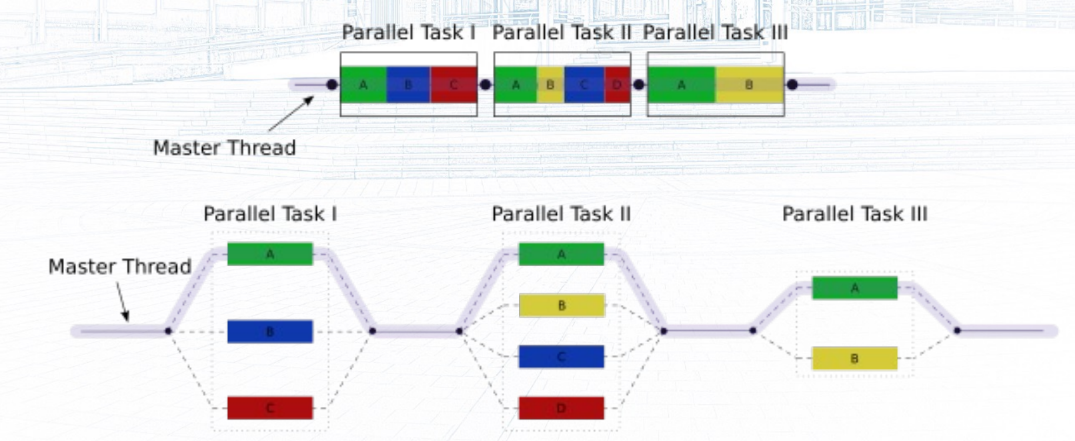
\includegraphics[width=0.8\textwidth]{ForkJoin.png}
    \caption{Fork-Join}
    \label{fig:ForkJoin}
\end{figure} 

\section{OpenMP memory }
\begin{itemize}
    \item \textbf{Shared memory model}: thread comunicano tramite accesso a variabili condivise.
    \item \textbf{La condivisione è definita sinitatticamente}: \begin{itemize}
                                                                    \item Ogni variabile che è vitsa da 2 o più threads è \textbf{condivisa}
                                                                    \item Ogni variabile che è vista da un solo thread è \textbf{privata}
                                                                \end{itemize}
    \item \textbf{Sono possibili le \texttt{Race Conditions}}: si usa la sincronizzazione per prevenire i confilitti e si cambia il modo di archiviazione dei dati per minimizzare la sincronizzazione
\end{itemize}

\newpage
\section{Sintassi}
È la direttiva che si usa all'inizio della sezione.
\begin{lstlisting}[style=cppstyle]
    #pragma omp <directive> [clause[,clause]...]
\end{lstlisting}

    \subsection{Direttive}
    \begin{itemize}
        \item \textbf{parallel}: crea un team di thread che eseguono il blocco di codice incluso in parallelo.
        \item \textbf{for}: suddivide un ciclo in iterazioni più piccole che possono essere eseguite in parallelo da thread diversi.
        \item \textbf{sections}: suddivide il blocco di codice incluso in diverse sezioni che possono essere eseguite in parallelo.
        \item \textbf{single}: specifica che un blocco di codice deve essere eseguito da un solo thread.
        \item \textbf{critical}: specifica che un blocco di codice deve essere eseguito da un solo thread alla volta.
        \item \textbf{atomic}: specifica che è necessario accedere a una variabile in modo atomico.
    \end{itemize}

\section{Controlling Granularity}
\begin{lstlisting}[style=cppstyle]
    #pragma omp parallel if (expression)
\end{lstlisting}
Può essere usato per disabilitare la parallel. in alcuni casi.
\\ \\
\begin{lstlisting}[style=cppstyle]
    #pragma omp num_threads (expression)
\end{lstlisting}
Controllare il numero di threads usati in questa regione parallel.

\newpage
\section{Data Environment}
\begin{itemize}
    \item \textbf{Shared Memory programming model}: la maggior parte delle variabili sono condivise per impostazione predefinita.
    \begin{lstlisting}[style=cppstyle]
        {
            int sum = 0;
            #pragma omp parallel for
            for(int i = 0; i < N; i++) sum += i;
        }\end{lstlisting}
    \item Alcune variabili possono essere private
\end{itemize}

\begin{figure}[h]
    \centering
    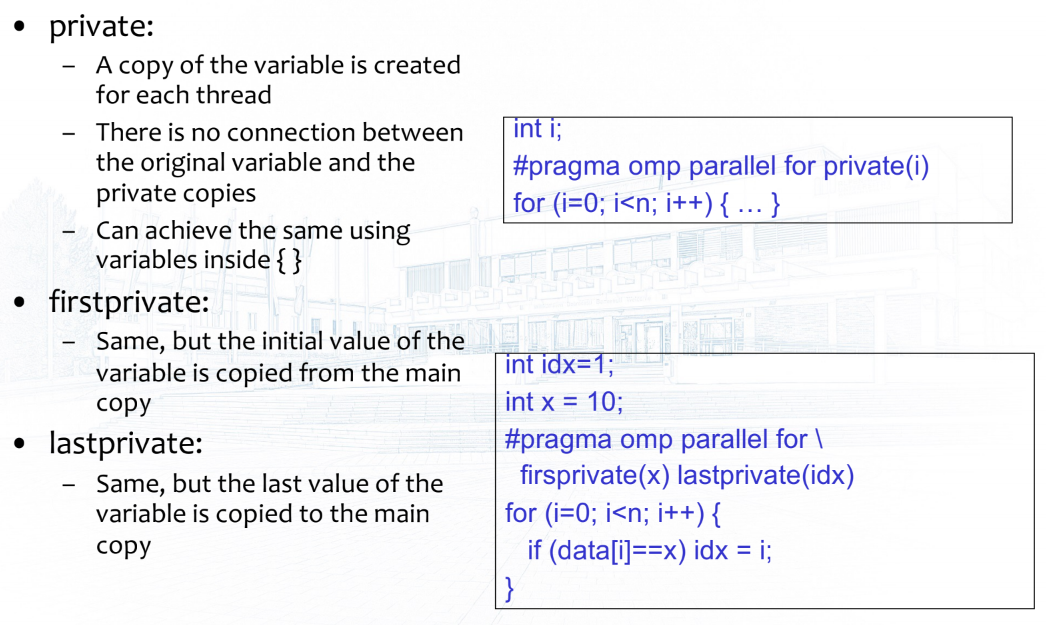
\includegraphics[width=0.6\textwidth]{private.png}
    \caption{Overriding storage attributes}
    \label{fig:OverridingStorageAttributes}
\end{figure}

\section{Synchronization Mechanism}
    \subsection{Single/Master execution}
    
\end{document}
